\documentclass[11pt,aspectratio=169]{beamer}
%%%%%%%%% GENERAL PACKAGES
%\usepackage[dvipsnames]{xcolor}
%\usepackage{pdfpages}
%\usetheme[progressbar=frametitle]{metropolis}
%\setbeamercolor{background canvas}{bg=white}
%\usepackage{appendixnumberbeamer}
%\usepackage{booktabs}
%\usepackage[scale=2]{ccicons}
%\usepackage{pgfplots}
%\usepgfplotslibrary{dateplot}
%\usepackage{xspace}
%\newcommand{\themename}{\textbf{\textsc{metropolis}}\xspace}
%\usepackage[absolute,overlay]{textpos}






%%%%%%%%% COLOR THEME

% Define some colors:
\definecolor{DarkFern}{HTML}{407428}
\definecolor{DarkCharcoal}{HTML}{4D4944}
\definecolor{AlertColor}{RGB}{89,124,158}
\definecolor{HighLight}{RGB}{96,95,134}
\definecolor{Important}{RGB}{234,122,133}
\definecolor{Yellow}{HTML}{00539C}
\colorlet{Fern}{DarkFern!85!white}
\colorlet{Charcoal}{DarkCharcoal!85!white}
\colorlet{LightCharcoal}{Charcoal!50!white}
\colorlet{HighLight2}{AlertColor}
\colorlet{DarkRed}{red!70!black}
\colorlet{DarkBlue}{blue!70!black}
\colorlet{DarkGreen}{green!70!black}
\definecolor{RoyalBlue}{HTML}{00539C}
\definecolor{Peach}{HTML}{EEA47F}
\definecolor{ForestGreen}{HTML}{2C5F2D}
\definecolor{MossGreen}{HTML}{E8FCC9}
\definecolor{SeaGreen}{HTML}{2E8B57}
% Use the colors:
\setbeamercolor{title}{fg=Fern}
\setbeamercolor{frametitle}{fg=MossGreen,bg=ForestGreen}
\setbeamercolor{normal text}{fg=Charcoal!70!black}
\setbeamercolor{block title}{fg=black,bg=Fern!25!white}
\setbeamercolor{block body}{fg=black,bg=Fern!10!white}
\setbeamercolor{block title alerted}{fg=black,bg=DarkRed!25!white}
\setbeamercolor{block body alerted}{fg=black,bg=DarkRed!10!white}
\setbeamercolor{alerted text}{fg=DarkRed}
\setbeamercolor{itemize item}{fg=Charcoal}



%%%%%%%%% OTHER COMMANDS
\newcommand{\indep}{\perp\!\!\! \perp}
\newcommand{\comment}[1]{}
\newcommand{\bs}{\boldsymbol}
\newcommand{\tr}{\text{trace}}
\newcommand{\sgn}{{\rm sgn}}
\def\T{\top}
%\newcommand{\det}{\text{det}}
\newcommand{\var}{\mathrm{var}}
\newcommand{\cC}{{\cal C}}
\renewcommand{\d}{{\rm d}}
\newcommand{\cG}{{\cal G}}
\newcommand{\cV}{{\cal V}}
\newcommand{\cE}{{\cal E}}
\newcommand{\cM}{{\cal M}}
\newcommand{\cP}{{\cal P}}
\newcommand{\cX}{{\cal X}}
\newcommand{\cY}{{\cal Y}}
\newcommand{\X}{\mathbf{X}}
\newcommand{\Y}{\mathbf{Y}}
\newcommand{\x}{\mathbf{x}}
\newcommand{\y}{\mathbf{y}}
\newcommand{\z}{\mathbf{z}}

\newcommand{\argmin}{\operatornamewithlimits{argmin}}
\newcommand{\eps}{\varepsilon}
\newcommand{\<}{\langle}
\renewcommand{\>}{\rangle}


%

\setbeamertemplate{navigation symbols}{}
\setbeamertemplate{footline}[text line]{%
    \hfill\strut{%
        \scriptsize\sf\color{black!60}%
        \quad\insertframenumber/\inserttotalframenumber
    }
    %\hfill
    }


\usenavigationsymbolstemplate{}
\setbeamersize{text margin left=.2cm,text margin right=.2cm} 
\addtobeamertemplate{frametitle}{}{\vspace{-1.2mm}}
\setbeamertemplate{itemize item}{$\bullet$}

\setbeamertemplate{itemize subitem}{\tiny\raise1.5pt\hbox{\donotcoloroutermaths$\blacktriangleright$}}
\setbeamertemplate{itemize subsubitem}{\tiny\raise1.5pt\hbox{\donotcoloroutermaths$\blacktriangleright$}}
\setbeamertemplate{enumerate item}{\insertenumlabel.}
\setbeamertemplate{enumerate subitem}{\insertenumlabel.\insertsubenumlabel}
\setbeamertemplate{enumerate subsubitem}{\insertenumlabel.\insertsubenumlabel.\insertsubsubenumlabel}
\setbeamertemplate{enumerate mini template}{\insertenumlabel}






\newcommand{\TODO}[1]{{\color{red}{[TODO: #1]}}}


\newcommand{\R}{\mathbb R}
\newcommand{\E}{\mathbb E}
\renewcommand{\P}{\mathbb P}


\DeclareMathOperator*{\cov}{cov}


\newsavebox{\zerobox}
\newenvironment{nospace}
{\par\edef\theprevdepth{\the\prevdepth}\nointerlineskip
  \setbox\zerobox=\vtop to 0pt\bgroup
  \hrule height0pt\kern\dimexpr\baselineskip-\topskip\relax
}
{\par\vss\egroup\ht\zerobox=0pt \wd\zerobox=0pt \dp\zerobox=0pt
  \box\zerobox}

\usepackage{soul}
\makeatletter
\let\HL\hl
\renewcommand\hl{%
  \let\set@color\beamerorig@set@color
  \let\reset@color\beamerorig@reset@color
  \HL}
  \makeatother

\usepackage{tikz}

%\usecolortheme{whale}

\title[Calculus and Linear Algebra]{Lecture 1 : Calculus}
\author[Piotr Zwiernik, Barcelona School of Economics]{Piotr Zwiernik \\ $\;$\\
Mathematics Brush-up\\ $\;$\\ $\;$\\

\includegraphics[width=1in]{img/bse.png}  
}
\date{}

%\beamerdefaultoverlayspecification{<+->}

\begin{document}
\begin{frame}
\titlepage
\end{frame}



%--------------- slide 2  ----------------%


%--------------- slide 1  ----------------%
\begin{frame}
\frametitle{Goal the course}
%\begin{small}
\textcolor{blue}{Review} basic tools that are useful in different areas of economics and finance.\\[6mm]

These tools will be \textcolor{blue}{crucial} for all the \textcolor{blue}{courses} of your program.\\[6mm]

\textcolor{blue}{Warm up} before the Master starts.\\[6mm]

\textcolor{blue}{Main references:} 
\begin{enumerate}
\item {\it Mathematics for Economists} by C. P. Simon and L. Blume

\item {\it Mathematics of Economics and Business} by F. Werner and Y. N. Sotskov
\end{enumerate}


%\end{small}
\end{frame}

\begin{frame}{Cultivate a Critical Mindset}
Technical knowledge requires effort. 
\begin{itemize}
  \item [$\bullet$] \textbf{If a step feels ``magical'', stop.} \\ 
        \quad Ask \emph{why} it works, not just \emph{how}.  \\[5mm]
        \smallskip
  \item [$\bullet$] \textbf{Challenge every answer - especially given by LLMs.} \\ 
        \quad Large-language models can sound confident yet be wrong;\\  
        \qquad always verify with first principles or a textbook.\\[5mm]
        \smallskip
  \item [$\bullet$] \textbf{Use multiple lenses.}\\  
        Check special cases, draw a picture, test with code, or look for a counter-example.
\end{itemize}
\end{frame}


\begin{frame}
\frametitle{Index}
%\begin{small}
\begin{enumerate}
\item Sequences and series
\item Functions of one variable
\item Differentiation
\item Integration
\item Vectors
\item Matrices and determinants
\item Systems of linear equations
\item Eigenvalue problems and quadratic forms
\item Functions of several variables
\item Introduction to differential equations
\end{enumerate}

%\end{small}
\end{frame}


\begin{frame}
\frametitle{Sequences }
%%\begin{small}
\textcolor{blue}{Sequence}: an infinite set of numbers arranged in a definite order. \\[3mm]

\textcolor{blue}{Notation:} $\{a_n\}_{n=1,2,3,...}$ where each $a_n$ is a real number.
\vskip12 pt
A sequence may be defined by a \textcolor{blue}{formula} or by a \textcolor{blue}{recursion}.
\vskip 12pt
\textcolor{blue}{Examples:} 
\begin{enumerate}
\item $a_n=\frac{n-1}{2n+1}$\quad  \begin{tiny}$(a_1=0, a_2=\frac15,a_3=\frac27,...)$ \end{tiny}

\item $a_1=2, \; a_{n+1}=2a_n-1$\quad  \begin{tiny}$(a_1=
2, a_2=3,a_3=5,...)$ \end{tiny}



\item $a_1=1, a_2=1, \; a_{n+1}=a_n+a_{n-1}$\quad  \begin{tiny}$(a_1=1, a_2=1,a_3=2,...)$ \end{tiny}



\item \alert{Arithmetic sequence}: $a_{n+1}=a_n+d$ or $a_n=a_1+(n-1)d$

$a_1$ is given, $d=$difference 


\item \alert{Geometric sequence}: $a_{n+1}=a_n  r$ or $a_n=a_1 r^{n-1}$

$a_1$ is given, $r=$ratio
\end{enumerate}
%%\end{small}
\end{frame}

\begin{frame}{}
%%\begin{small}
Sequences arise in many economic applications, e.g. in \textcolor{blue}{economics of finance and investment}.
\vskip 12pt
Sequences help to understand the concept of a \textcolor{blue}{limit of a function} and the significance of the \textcolor{blue}{number $e$}. 
\vskip 12pt
 They are also important when solving \textcolor{blue}{difference equations}.
\vskip 12pt
\textcolor{blue}{Read} Chapter 2 of Werner-Sotskov 
\vskip 12pt
 \textcolor{blue}{Exercises:} 2.4, 2.5, 2.7 (Werner-Sotskov)
%%\end{small}
\end{frame}



\begin{frame}
\frametitle{Economic examples  }
%\begin{small}
\begin{enumerate}
\item {Invest} an amount $P$(principal) at an \textcolor{blue}{annual interest rate} $R$. After $n$ years the total amount is the \textcolor{blue}{geometric sequence}
$$a_n=P(1+R)^n\qquad (\text{ratio}=1+R, a_1=P(1+R))$$
\textcolor{blue}{Example}: $P=1000$ euros, $R=8\%$, $a_1=1080$, $a_{50}\approx 46901$.

The annual interest rate $R$ is also called \alert{annual percentage rate} (APR).

%
%\begin{tiny} In practice financial institutions pay interest more frequently...\end{tiny}

\item \textcolor{blue}{Compounded interest:} If instead the bank pays interests \textcolor{blue}{$m$ times a year}, after $n$ years, we obtain
$$
a_n=P\left(1+\frac{R}{m}\right)^{n m}\qquad (\text{ratio}=(1+\frac{R}{m})^{m})
$$

\textcolor{blue}{Example}: $P=1000$ euros, $R=8\%$, $m=4$, $a_1=1082.43$. 

The investment grows $8.243 \%$ in one year, which is called the \alert{equivalent annual rate} (EAR), that is, the rate that compounded annually, gives the same yield.

\end{enumerate}
%\end{small}
\end{frame}

\begin{frame}{}
%\begin{small}
\begin{enumerate}
\item[] \textcolor{blue}{Remark}:  EAR does not depend on $P$ or $n$. In fact, it is equal to
$$
\left( 1+\frac{R}{m}\right)^m-1.
$$

\textcolor{blue}{Example}: if the bank pays an interest monthly ($m=12$) at an APR of $6\%$, then the EAR is 6.17$\%$

\vskip 12pt

\item[3.] The \textcolor{blue}{Present Discounted Value} of an amount $A$ to be received in $n$ years at an annual interest rate $R$ is
$$
a_n=\frac{A}{(1+R)^n}
$$

\textcolor{blue}{Example}: would you prefer $1000$ euros now or 1050 in one year? It depends on $R$! \end{enumerate}
%\end{small}
\end{frame}


\begin{frame}
\frametitle{Properties of a sequence}
%\begin{small}
 A sequence is  \textcolor{blue}{increasing} if for every $n$, $a_{n+1} \geq a_n$, and \textcolor{blue}{strictly increasing} if $a_{n+1}  >a_n$. \begin{tiny} (which is equivalent to $a_{n+1}-a_n>0$, or $\frac{a_{n+1}}{{a_n}}>1$ if $a_n>0$) \end{tiny}
\vskip 12pt
A sequence is \textcolor{blue}{decreasing} if for every $n$, $a_{n+1} \leq a_n$, and \textcolor{blue}{strictly decreasing} if $a_{n+1}  <a_n$.
\vskip 12pt
A sequence is (strictly) \textcolor{blue}{monotone} if it is (strictly) increasing or (strictly) decreasing.
\vskip 12pt
It is \textcolor{blue}{bounded} if there exists a constant $C>0$ such that,
for all  $n$, $a_{n} \in [-C, C]$.
\vskip 12pt
\textcolor{blue}{Examples:} 
\begin{enumerate}
\item $a_n=2(n-1)^2-n$ is strictly increasing \begin{tiny} (since $a_{n+1}-a_n=4n-3>0$)\end{tiny}

\item $a_n=\frac{1}{n^2}$ is bounded\begin{tiny} (since $a_n \in [-1,1])$\end{tiny}
\end{enumerate}
\end{frame}

{
\begin{frame}[plain]
\noindent
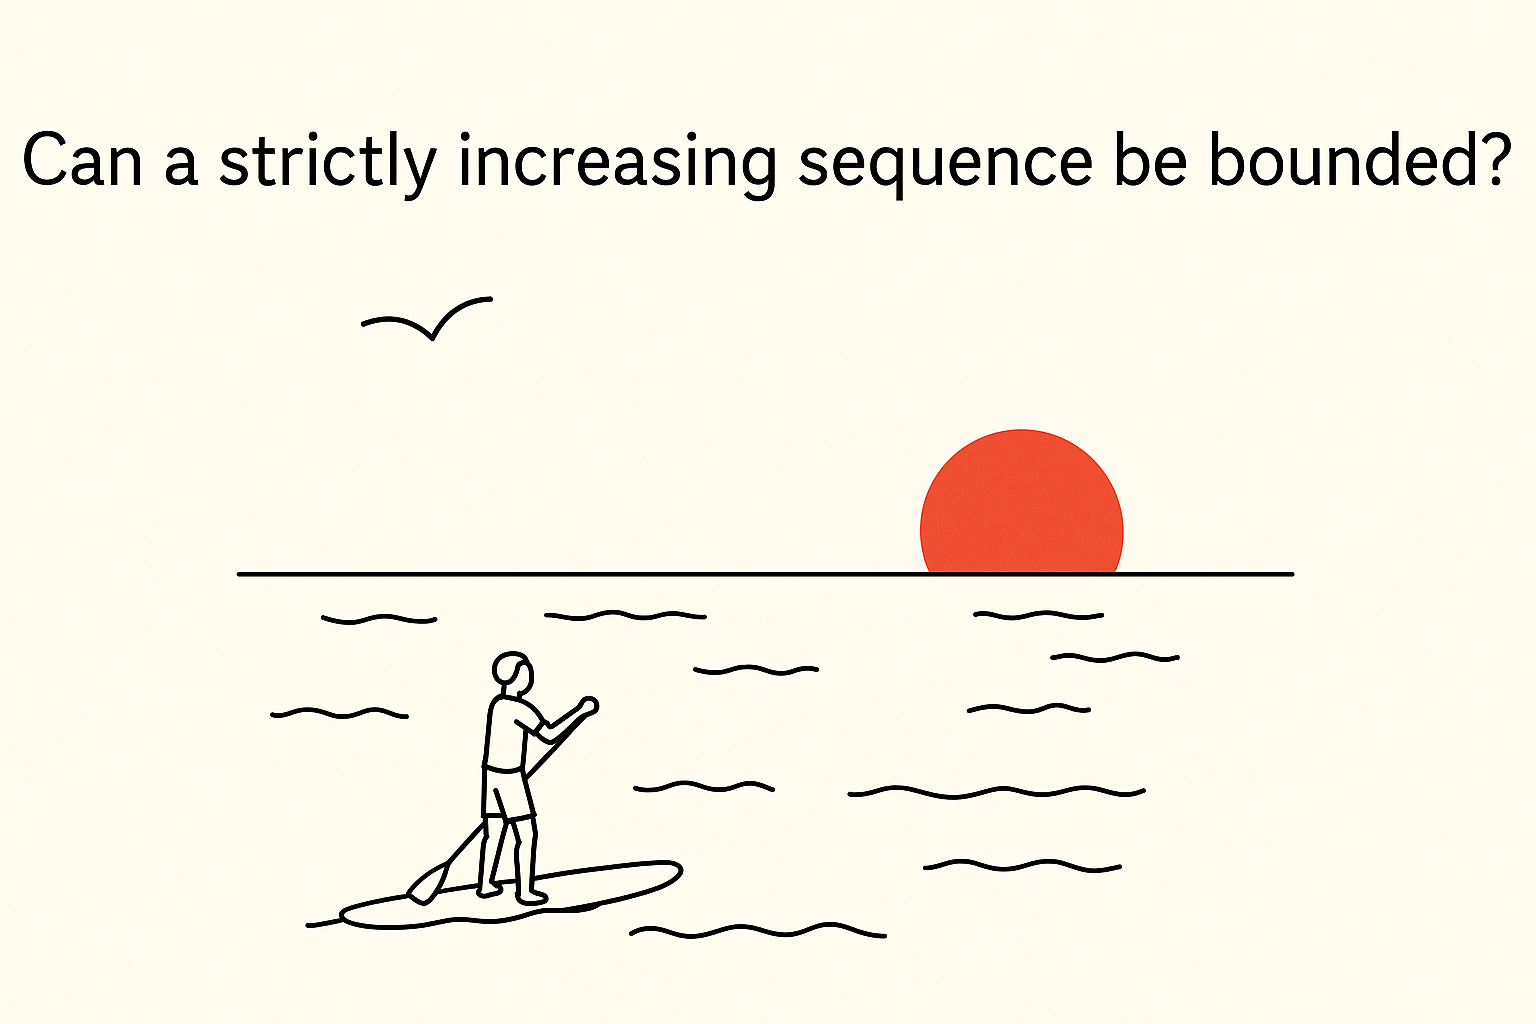
\includegraphics[scale=.25]{vbreaks/question1.png}
\end{frame}
}


\begin{frame}
\frametitle{Limit of a sequence}


 A finite number $a$ is called the \alert{limit} of a sequence $\{a_n\}$ if as $n$ gets larger, $a_n$ gets closer to $a$. \textcolor{blue}{Notation:} \hl{$\lim_{n \rightarrow \infty} a_n=a$}.
\vskip 12pt
A sequence is said to be \textcolor{blue}{convergent} if it has a limit. Otherwise, we say that it has \textcolor{blue}{no limit} or  \textcolor{blue}{diverges} (when the limit is $\infty$ or $-\infty$).

\vskip 12pt
\textcolor{blue}{Examples} 
\begin{enumerate}
\item $a_n=\frac{1}{n^2}$ is convergent to 0

\item $a_n=(-1)^n$ has no limit

\item $a_n=n^2$ diverges

\item $a_n=r^n$ converges to $0$ if  $\vert r \vert <1$, diverges if $r>1$ and has no limit if $r\leq -1$.

\end{enumerate}

 


%\end{small}
\end{frame}

\begin{frame}
\frametitle{Limit of a sequence}
%\begin{small}
\begin{alertblock}{Definition: $a$ is a limit of the sequence $\{a_n\}$\;\; $(\lim_{n\to \infty}a_n=a$)}
\qquad\qquad$
\forall \epsilon >0 \;\;\; \exists N_{\epsilon}>0\;\;\; s.t\;\;\;\;\;\forall n>N_{\epsilon}\quad\quad \vert a_n-a \vert < \epsilon.
$	
\end{alertblock}

 \textcolor{blue}{Example:}  the sequence $a_n=\frac{1}{n}$ is convergent to 0. \\[3mm]
\qquad Indeed. For each $\epsilon>0$ take any $N_{\epsilon}>\frac{1}{\epsilon}$. \\[2mm]
 \textcolor{blue}{Check from definition:} 
 \begin{itemize}
 	\item $\lim_{n\to\infty} a_n=a$ is the same as $\lim_{n\to \infty} |a_n-a|=0$\\[2mm]
 	\item If $a_n=a$ for all $n$ then $\lim_{n\to\infty}a_n=a$.
 \end{itemize}
%\end{small}
\begin{block}{If formal definition hard to work with, try to use \alert{bounds} instead, e.g.}
$$
0\;<\;\tfrac{1}{2n^2-1}\;\leq\; \tfrac{1}{n}, \quad n \geq 1 \quad \mbox{{(\small and so the middle sequence converges to zero)}	}.
$$
\end{block}
\end{frame}

\begin{frame}
\frametitle{Limit of a sequence}
%\begin{small}
\textcolor{blue}{More Examples} 
\begin{enumerate}

\item The sequence $\left(1+\frac{1}{n}\right)^n$ converges to the number $e$  $(\approx 2.71828)$ 
\item The sequence $\left(1+\frac{x}{n}\right)^n$ converges to $e^x$, for any $x$. \begin{tiny}We will see a proof of these facts using integrals.  \end{tiny}
\end{enumerate}


\textcolor{blue}{Economic example:} if the interest is \textcolor{blue}{compounded continuously} at an APR of $R$, the return after $n$ years on an initial amount $P$ is 
$$
\lim_{m\rightarrow \infty} P\left(1+\frac{R}{m}\right)^{n m}=P e^{Rn}
$$ 
and the present discounted value of an amount $A$ received in $n$ years is $A e^{-Rn}$. 
\vskip 12pt
\textcolor{blue}{Example:} if the interest is compounded continuously at an APR of $8\%$, then the EAR is $8.329\%$ \begin{tiny}(since $e^{0.08}-1=0.08329$) \end{tiny}  


%\end{small}
\end{frame}

\begin{frame}
\frametitle{Limit of a sequence}
%\begin{small}
\textcolor{blue}{Theorem:} Every bounded and monotone sequence is convergent. \\\begin{tiny} (useful to show convergence but not to compute limits) \end{tiny}
\vskip 12pt
\textcolor{blue}{Remark:} Observe that only bounded  \begin{tiny}(for example $a_n=(-1)^n$)\end{tiny} or only monotone  \begin{tiny}(for example $a_n=n$)\end{tiny} is not sufficient for being convergent.

\vskip 12pt

\textcolor{blue}{Example:} the sequence $a_1=1, \; a_{n+1}=\sqrt{3a_n}$ is bounded by $3$ \begin{tiny} (proof by induction) \end{tiny} and strictly increasing \begin{tiny} (since $\frac{a_{n+1}}{a_n}>1$)\end{tiny}, thus convergent.

\begin{tiny}Write a couple of first entries of the sequence. Using geometric series show that this sequence converges to $3$.  \end{tiny}
\vskip 12pt

\textcolor{blue}{Theorem:} If $\lim_{n \rightarrow \infty} a_n=a$ and $\lim_{n \rightarrow \infty} b_n=b$
then $$\lim_{n \rightarrow \infty} (a_n+b_n)=a+b, \quad\lim_{n \rightarrow \infty} a_nb_n=ab,
\quad\lim_{n \rightarrow \infty} \frac{a_n}{b_n}=\frac{a}{b},$$
the last equality being true only if $b_n,b\neq0$.
 


%\end{small}
\end{frame}

\begin{frame}
\frametitle{Partial sums}
%\begin{small}
The \textcolor{blue}{nth partial sum $s_n$} of a sequence $\{a_n\}$ is defined as the sum of the first $n$ terms:
$$
s_n\;\;=\;\;a_1+\cdots+a_n\;\;=\;\;\sum_{k=1}^n a_k.
$$

\textcolor{blue}{Examples} 
\begin{enumerate}
\item If $a_n=3+(-1)^n \frac{2}{n}$ then
$
s_1=1, s_2=5, s_3=\frac{22}{3},\dots
$

\begin{tiny}$(a_1=1, a_2=4,a_3=\frac73,...)$ \end{tiny}

\item The nth partial sum of an \textcolor{blue}{arithmetic sequence} is $$s_n=n a_1+\frac{n(n-1)}{2}d.$$



\item The nth partial sum of a \textcolor{blue}{geometric sequence} with ratio $r \neq 1$ is $$s_n=a_1 \frac{1-r^n}{1-r}.$$
\begin{tiny}These formulas can help to compute the limit of a sequence\end{tiny}
\end{enumerate}


%\end{small}
\end{frame}

\begin{frame}
\frametitle{Economic example }
%\begin{small}
\textcolor{blue}{Regular savings:} We \textcolor{blue}{invest} an amount $A$ at the beginning of every year at an \textcolor{blue}{annual interest rate} $R$. After $n$ years the total amount is given by the \textcolor{blue}{geometric partial sum} 

\begin{align*}
s_n&=A(1+R)^n+A(1+R)^{n-1}+\cdots+A(1+R)\\
&= A(1+R)\frac{(1-(1+R)^n)}{1-(1+R)}\\
&=\frac{A(1+R)}{R}((1+R)^n-1)
\end{align*}
\begin{tiny} Here $a_1=A(1+R)$ and $r=1+R$\end{tiny}
%\end{small}
\end{frame}

\begin{frame}
\frametitle{Series and convergence of series}
%\begin{small}
The sequence $\{s_n\}$ of partial sums of a sequence $\{a_n\}$ is called a \textcolor{blue}{series}. 
\vskip 12pt
A series $\{ s_n\}$ is said to converge if it has a limit $s$. In this case, the value $s$ is called the \textcolor{blue}{sum} of the series:
$$
s=\lim_{n \rightarrow \infty} s_n=\lim_{n \rightarrow \infty} \sum_{k=1}^n a_k
=\sum_{k=1}^{\infty} a_k.
$$
\vskip 12pt
\textcolor{blue}{Example:} The series associated to a  geometric sequence is called a \textcolor{blue}{geometric series} which converges if and only if $\vert r \vert <1$, and in this case,
$$
s=\sum_{k=1}^{\infty} a_1 r^{k-1}=\lim_{n \rightarrow \infty}
a_1 \frac{1-r^n}{1-r}=\frac{a_1}{1-r}. 
$$


%\end{small}
\end{frame}


\begin{frame}[plain] % "plain" removes header/footers
  \centering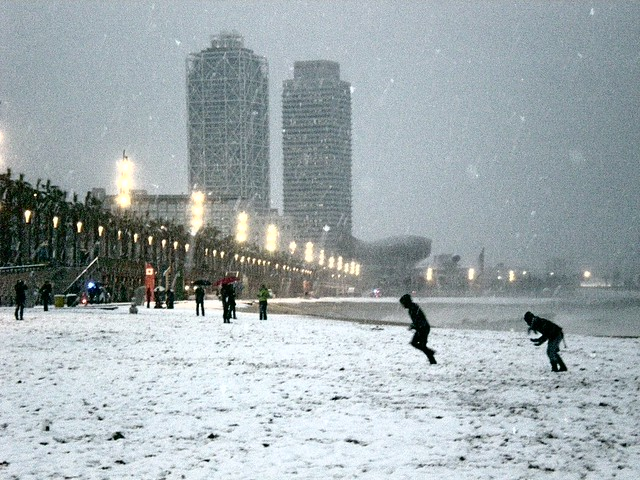
\includegraphics[height=\paperheight]{vbreaks/vb2.jpg}
\end{frame}





\begin{frame}
\frametitle{Chapter 2: Functions of one variable}
%\begin{small}


A \textcolor{blue}{one variable function} is simply a mapping that assigns a unique number $y$ in $\R$ to each number $x$ in $\R$. We write $f(x)=y$. 
\vskip 12pt
$x$ is called the independent variable, or in economic applications, \textcolor{blue}{exogenous variable}, and $y$ is called the dependent variable or \textcolor{blue}{endogenous variable}.
\vskip 12pt
\textcolor{blue}{Economic examples:} endogenous variables: cost, revenue, profit, demand, production, utility, etc. and exogenous variables: time, labor, capital, price, etc.
\vskip 12pt
\textcolor{blue}{Read} Chapter 3 of Werner-Sotskov and Sections 2.1, 2.2, 5.1, 5.2, 5.3 of Simon-Blume
%\end{small}
\end{frame}

\begin{frame}
\frametitle{Graph and domain}
%\begin{small}
\begin{block}{Definition}
The \textcolor{blue}{graph} of a functions consists of all points $(x,y)$ in $\R^2$ such that $y=f(x)$.
\vskip 12pt
The \textcolor{blue}{domain} $D$ of a function are the numbers $x$ at which $f(x)$ is defined. \\[5mm]\textcolor{blue}{Notation} Write \hl{$f:D \rightarrow \R$}.	
\end{block}
\bigskip

\textcolor{blue}{Example}: The domain of the function $f(x)=\frac{1}{x}$ is $D=\R \setminus \{0\}$. 
\vskip 12pt
Sometimes it is interesting to consider a function in a \textcolor{blue}{restricted domain}.

%\end{small}
\end{frame}


\begin{frame}{
Properties of functions}
A function $f:D \rightarrow \R$ is called \textcolor{blue}{increasing} if 
$$
f(x_1)\leq f(x_2) \qquad \text{ for any } x_1<x_2,\quad  x_1,x_2 \in D,
$$
 and \textcolor{blue}{strictly increasing} if the sign is $<$. An increasing function is also called \textcolor{blue}{non-decreasing}.
\vskip 12pt
 A function $f:D \rightarrow \R$ is called \textcolor{blue}{decreasing} if $$
f(x_1)\geq f(x_2) \qquad \text{ for any } x_1<x_2, x_1,x_2 \in D,
$$ and \textcolor{blue}{strictly decreasing} if the sign is $>$.
A decreasing function is also called \textcolor{blue}{non-increasing}.
\vskip 12pt
 A function $f:D \rightarrow \R$ is called \textcolor{blue}{bounded} if there exists a constant $C>0$ such that
$$\vert f(x) \vert \leq C,\quad \text{for any } x \in D.$$ 
\end{frame}

\begin{frame}{Convex/concave functions}
%\begin{small}
If $x_1<x_2$ are two points in $\R$, the points of the form 
$$t x_1+(1-t)x_2,$$ where $t \in [0,1]$ are called the \textcolor{blue}{convex combination} of $x_1$ and $x_2$.\\ {\scriptsize (They give all the points lying in the interval $[x_1,x_2]$)}

\vskip 12pt
A set $D\subset \R$ is \textcolor{blue}{convex} if the convex combination of any $x_1,x_2 \in D$ lies in $D$.
\vskip 12pt
A function $f:D \rightarrow \R$, where $D$ is convex is called \textcolor{blue}{convex} (resp. \textcolor{blue}{concave}) if for every  $x_1,x_2 \in D$ and $t \in [0,1]$, 
$$f(t x_1+(1-t)x_2)\leq t\, f(x_1)+(1-t) f(x_2)$$
(resp. $\geq$). If for $t \in (0,1)$ and $x_1 \neq x_2$ the sign $<$ (resp. $>$) holds then it is \textcolor{blue}{strictly convex} (resp. \textcolor{blue}{strictly concave}).
\end{frame}

\begin{frame}
\frametitle{Convex function}

\begin{figure}
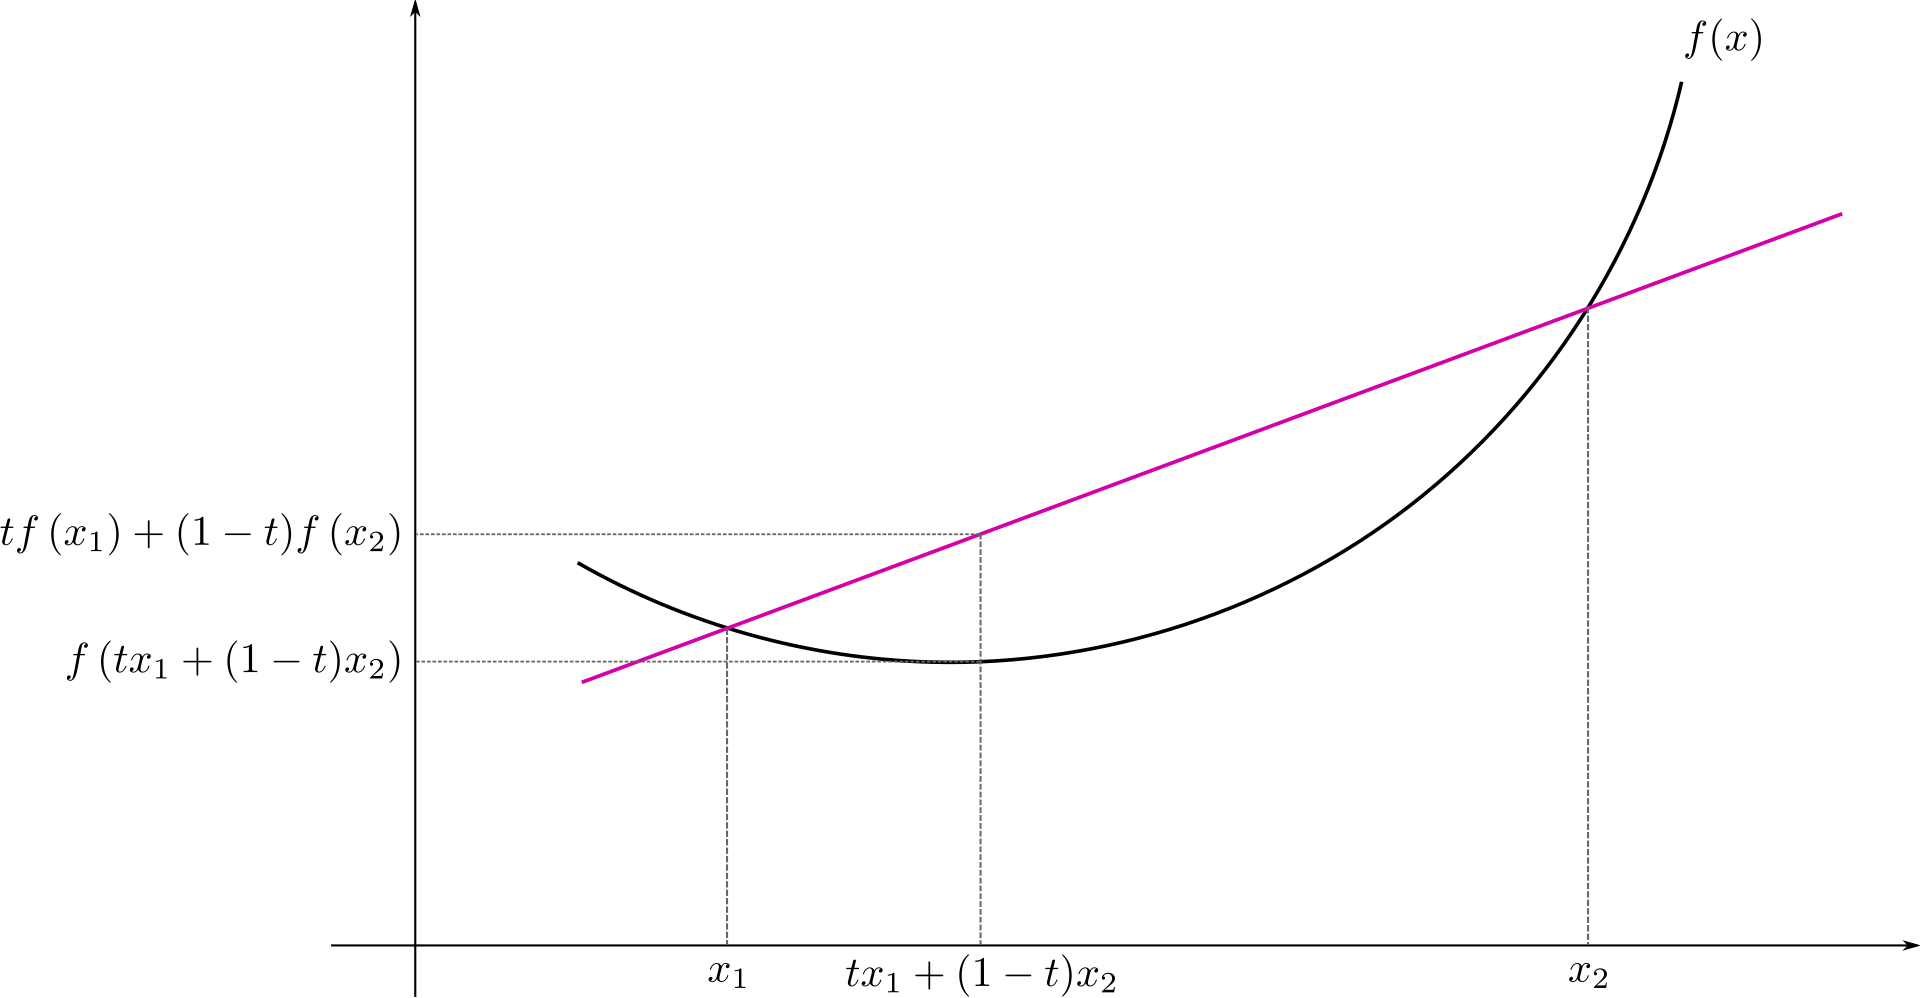
\includegraphics[width=4in]{img/convex} 
\end{figure}


\end{frame}

\begin{frame}{Quasi-convex/concave functions}
%\begin{small}

A function $f:D \rightarrow \R$, where $D$ is convex is called \textcolor{blue}{quasi convex} if for every  $x_1,x_2 \in D$ and $t \in [0,1]$, 
$$f(t x_1+(1-t)x_2)\leq \max(f(x_1), f(x_2)).$$


Similarly, \textcolor{blue}{quasi concave} means that
$$f(t x_1+(1-t)x_2)\geq \min(f(x_1), f(x_2)).$$

\vskip 12pt
\textcolor{blue}{Remark:} every convex function is quasi convex and every concave function is quasi concave.
\vskip 12pt

\textcolor{blue}{Theorem:} any strictly increasing function is quasiconvex and quasiconcave.

\begin{tiny} Proof: if $x_1<x_2$ then $f(x_1) \leq f(t x_1+(1-t)x_2)\leq f(x_2)$.\end{tiny}
%\end{small}
\end{frame}

\begin{frame}{Economic example: logistic growth function}
The standard logistic growth function is: 
$f(t) = \frac{L}{1 + e^{-k(t - t_0)}}$.\\[3mm]
\begin{minipage}{6cm}{}
	\begin{figure}
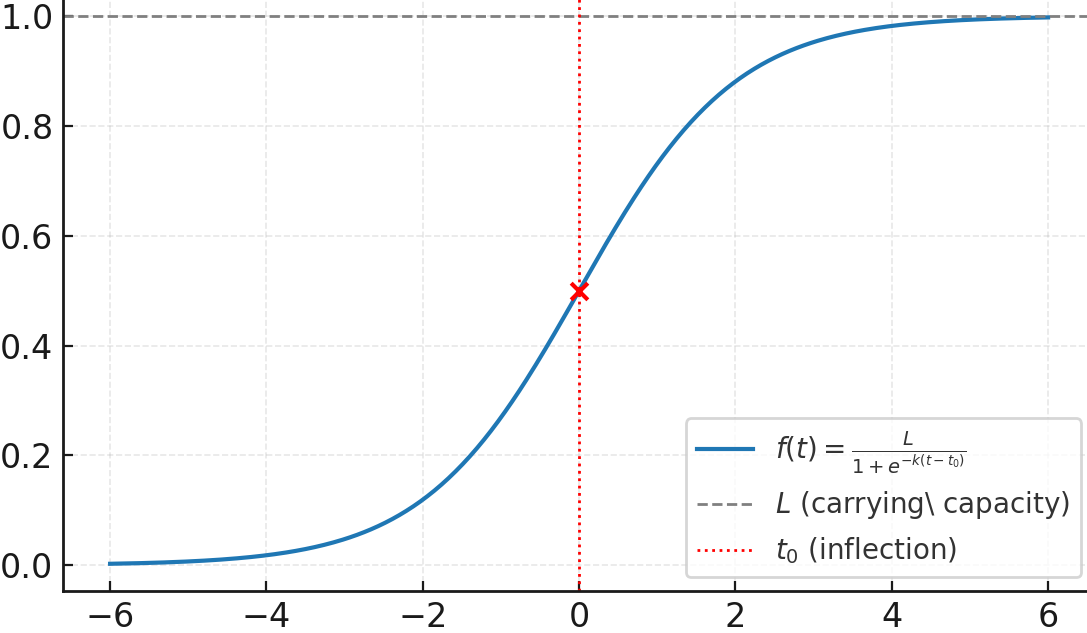
\includegraphics[width=2in]{img/returns1.png} 
\end{figure}
\end{minipage}\begin{minipage}{9cm}{}
	It satisfies:
	\begin{itemize}
		\item Initial phase: roughly exp. growth when $x \ll x_0$,
		\item Midpoint: $f(t_0) = L/2$,
		\item Saturation: approaches $L$ as $t \to \infty$.
	\end{itemize}
	(in the plot $L = 1, k = 1, and t_0 = 0$)
\end{minipage}

Interpretation: At first, the rate of increase increases, but after some point it slows down, and eventually decreases  until it reaches some level. 
\end{frame}

\begin{frame}{Economic example}
%\begin{small}
The logistic growth function is used to describe \textcolor{blue}{epidemic growth models}.  Check the following prediction versus epidemic curves over time of the  COVID-19 in China.
%\end{small}
\begin{figure}
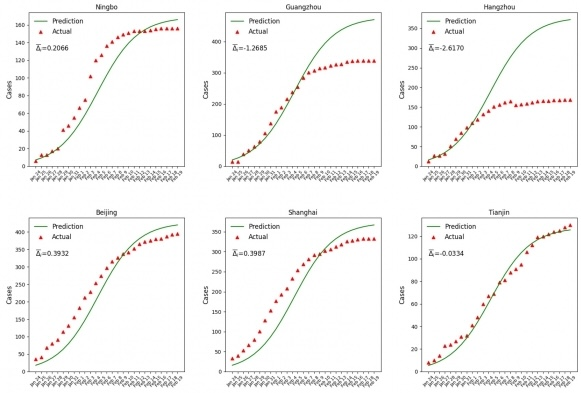
\includegraphics[width=0.60\textwidth]{img/figure}
\end{figure}
\end{frame}

\begin{frame}[plain]{Do you recognize this function?}
\begin{tikzpicture}[remember picture,overlay]
  % Base image (centered; name it if you want to reference it later)
  \node[inner sep=0,anchor=center,yshift=-0.07\paperheight] (bg) at (current page.center)
       {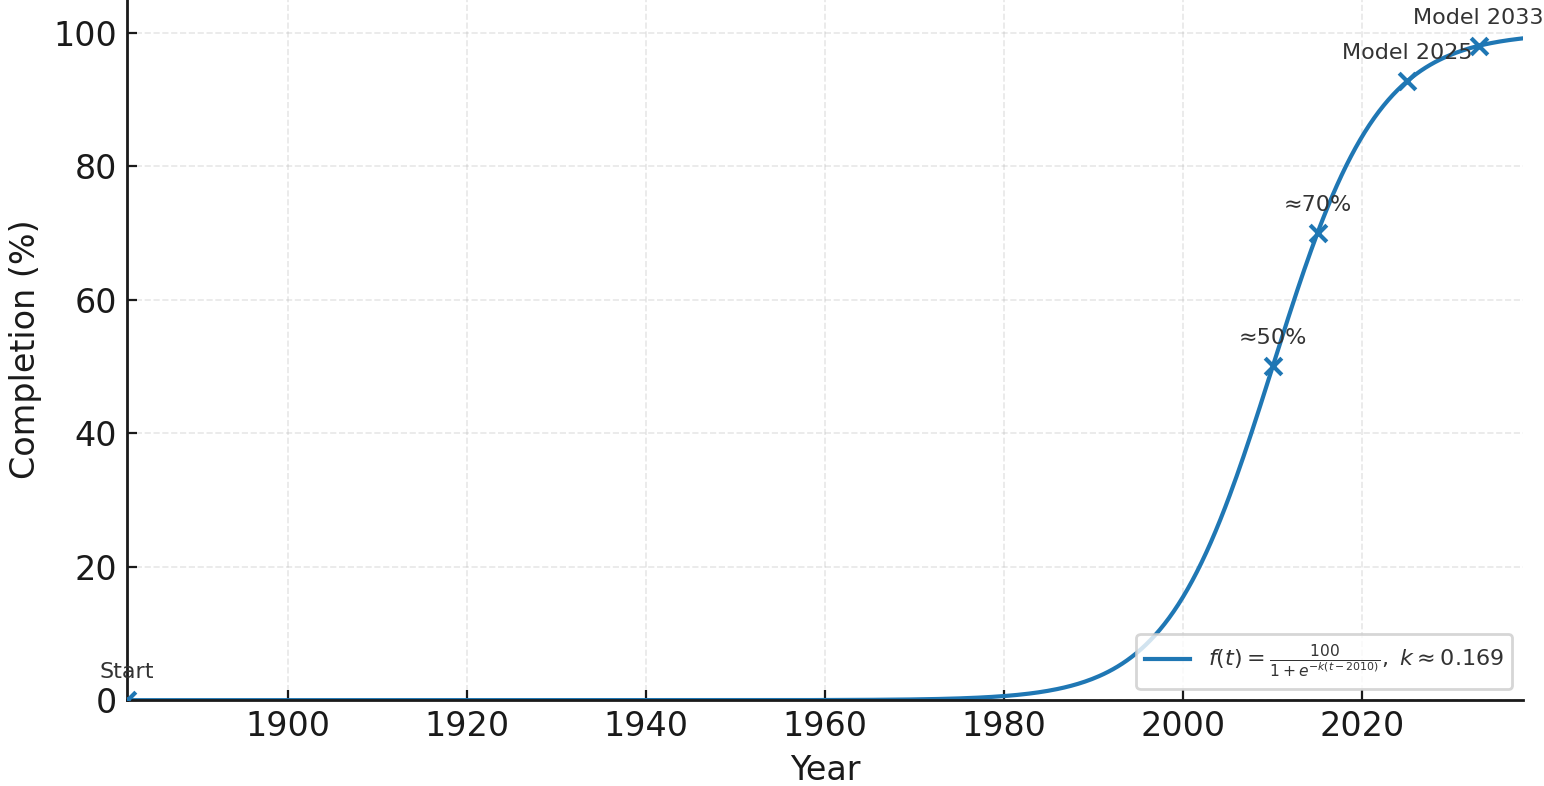
\includegraphics[scale=0.7]{img/SFprogress0.png}};

  % Overlay image: place relative to page, with fine offsets
 \only<2>{ \node[anchor=north west,
        xshift=0.2\paperwidth, % move right
        yshift=-0.18\paperheight] % move down
        at (current page.north west)
       {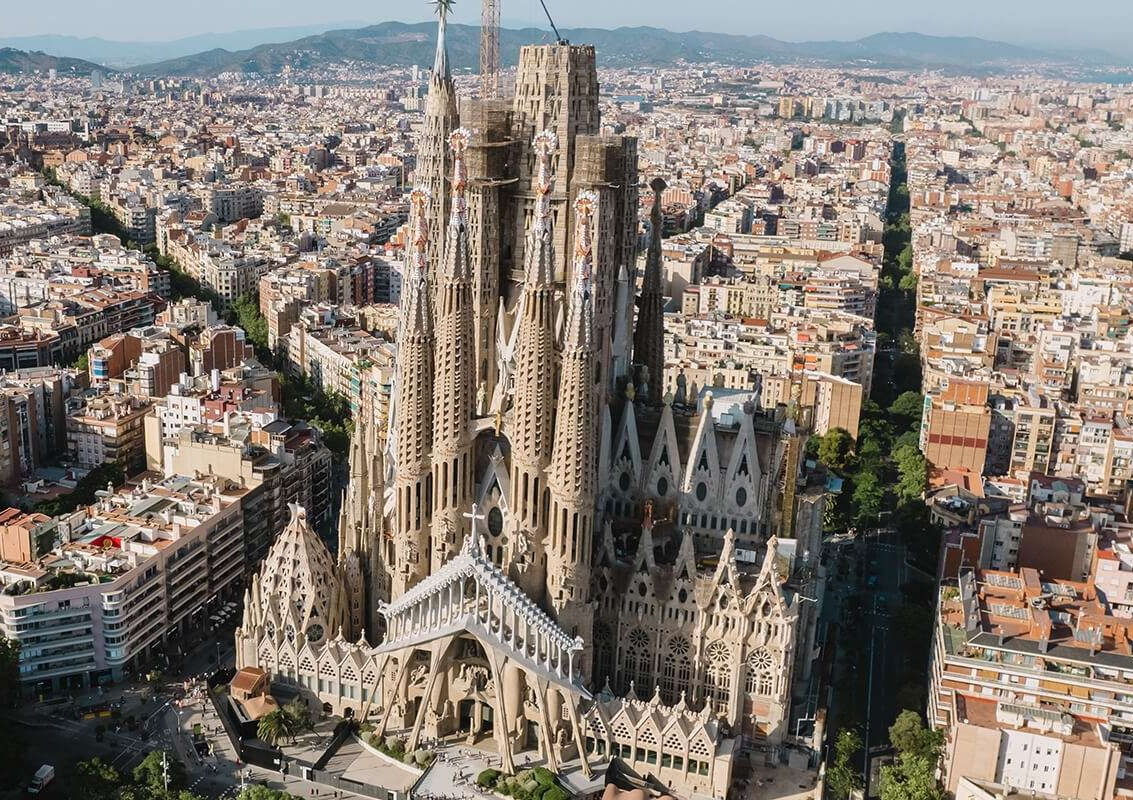
\includegraphics[width=0.45\paperwidth]{img/SF.jpg}};}
\end{tikzpicture}
\end{frame}

\begin{frame}
\frametitle{Examples of functions}
%\begin{small}
\begin{enumerate}
\item \textcolor{blue}{monomials}: $f(x)=a x^k$, $k$ natural number.

\item \textcolor{blue}{polynomials}: sums of monomials

\item \textcolor{blue}{rational functions}: ratios of polynomials

\item \textcolor{blue}{exponent functions}: $f(x)=a^x$

\item \textcolor{blue}{trigonometric functions}: $\sin(x)$, $\cos(x)$, etc.

\item \textcolor{blue}{linear functions}: $f(x)=mx+b$, \begin{tiny}($m$=slope and $(0,b)$=intercept) 

(linear functions also write as $y-f(x_0)=m(x-x_0)$)
\end{tiny} 

\item \textcolor{blue}{exponential function}: $f(x)=e^x$ \begin{tiny}(recall this is the limit of the sequence $\left(1+\frac{x}{n}\right)^n$)  \end{tiny} 

\item \textcolor{blue}{base e logarithm function}: $f(x)=\log x$ \begin{tiny}(defined as the unique function such that $e^{\log (x)}=x$ and $\log(e^x)=x$)  \end{tiny} 

\qquad \textcolor{blue}{recall:} $e^{x+y}=e^x e^y$, $e^0=1$,\\ \qquad\quad\qquad $\log(xy)=\log(x)+\log(y)$, $\log(1)=0$, $\log(a^x)=x\log(a)$.
\end{enumerate}

%\end{small}
\end{frame}

\begin{frame}
\frametitle{Exponential functions}
\begin{figure}
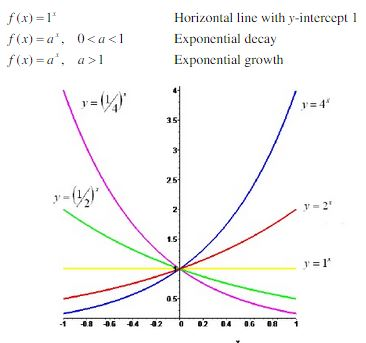
\includegraphics[width=2.5in]{img/exp} 
\end{figure}
\end{frame}

\begin{frame}
\frametitle{Chapter 3: Differentiation}
%\begin{small}
 \textcolor{blue}{Differentiation} gives information on how the function changes with respect to small changes of the independent variable.
\vskip 12pt
\textcolor{blue}{Example:} how does the change of the price of some product affect the amount of product customers will buy ?
\vskip 12pt
Differential calculus gives also information about extreme points, monotonicity, and convexity.
\vskip 12pt
\textcolor{blue}{Read} Chapter 4 of Werner-Sotskov, Chapters 2 to 5 of Simon-Blume
\vskip 12pt
\textcolor{blue}{Exercises:} 4.6(c), 4.10, 4.14, 4.15(a)-(c), 4.16(d), 4.17(b) (Werner-Sotskov), 5.5 (b)-(c)-(e) (Simon-Blume)


%\end{small}
\end{frame}


\begin{frame}
\frametitle{Limit of a function}
\begin{alertblock}{}
Let $f:D  \rightarrow \R$ and let $x_0 \in \R$. We say that $L$ is the l\textcolor{blue}{imit} of $f$ as $x$ tends to $x_0$ if for any sequence $\{x_n\} \in D$ convergent to $x_0$, the sequence
$\{f(x_n)\}$ converges to $L$. 	\\[3mm]
\textcolor{blue}{Notation:} $\lim_{x \rightarrow x_0} f(x)=L$. \textcolor{blue}{Remark:} we do note need that $x_0 \in D$.
\end{alertblock}
 \textcolor{blue}{Example:} $\lim_{x \rightarrow 0} x \sin\frac{1}{x}=0$ since $0\leq \vert x \sin\frac{1}{x}\vert \leq \vert x \vert$.
\begin{block}{Theorem}
	If $\lim_{x \rightarrow x_0} f(x)=y_1$ and $\lim_{x \rightarrow x_0} g(x)=y_2$,
then $$\lim_{x \rightarrow x_0} (f(x)+g(x))=y_1+y_2, \quad\lim_{x \rightarrow x_0} f(x)g(x)=y_1y_2,
\quad\lim_{x \rightarrow x_0} \frac{f(x)}{g(x)}=\frac{y_1}{y_2},$$
the last equality being true only if $y_2\neq0$ and $g(x) \neq 0$ around $x_0$.
\end{block}
%$$\lim_{x \rightarrow x_0} \sqrt{f(x)}=\sqrt{y_1}, \quad\lim_{x \rightarrow x_0} [f(x)]^n=y_1^n,
%\quad\lim_{x \rightarrow x_0} a^{f(x)}=a^{y_1}.$$

%\end{small}
\end{frame}

\begin{frame}{Continuity of a function}
%\begin{small}
\begin{alertblock}{Definition}
We say that a function $f$ is \textcolor{blue}{continuous}
at $x_0 \in D$ if $$\lim_{x \rightarrow x_0} f(x)=f(x_0).$$
If $f$ is continuous at every point of a set $B\subset D$, then we say that $f$ is continuous
at $B$.	
\end{alertblock}

\textcolor{blue}{Theorem:} If $f,g$ are continuous at $x_0$ then so are $f+g$ and $f g$. If moreover,
$g(x)\neq 0$ around $x_0$, then $\frac{f}{g}$ is continuous at $x_0$.

\vskip 12pt
\textcolor{blue}{Theorem:} If $f:[a,b] \rightarrow \R$ is continuous then it is bounded.

%\end{small}
\end{frame}


\begin{frame}{Continuity of a function}
%\begin{small}
The \textcolor{blue}{composition} of two functions $f$ and $g$ is the function  defined as
$h(x)=f(g(x))$, for all $x \in D_g$. 
\textcolor{blue}{Notation:} $h=f \circ g$.
\begin{block}{}
	If $f$ and $g$ are continuous, so is $h=f\circ g$. \\[3mm]
	\qquad Moreover, $\lim_{x\to x_0} f(g(x))=f(\lim_{x\to x_0}g(x))$.
\end{block}


%\begin{tiny} (For example, $g(x)$ can be the production function in terms of labor and $f$ the profit function in terms of production, then $h$ is the profit function in terms of labor) \end{tiny}
\vskip 12pt
Let $f:[a,b] \rightarrow \R$ be a \textcolor{blue}{strictly monotone continuous function} with $f(a)=c$ and $f(b)=d$.  We define the \textcolor{blue}{inverse function} of $f$ as the function $f^{-1}:[c,d] \rightarrow [a,b]$ such that $f \circ f^{-1}=\text{id}$ and $f^{-1} \circ f=\text{id}$.
\begin{block}{}
	If $f$ is strictly monotone continuous function, so is $f^{-1}$. 
\end{block}

\begin{tiny} (For example, $e^{\log(x)}=x$ and $\log(e^x)=x$.) \end{tiny}


%\end{small}
\end{frame}

\begin{frame}{Derivative}
%\begin{small}
Let $f:(a,b) \rightarrow \R$. The function $f$ is said to be \textcolor{blue}{differentiable} at $x \in (a,b)$ if the limit
$$
\lim_{h \rightarrow 0} \frac{f(x+h)-f(x)}{h},
$$
exists. In this case, it denoted $f'(x)$ and called the \textcolor{blue}{derivative} of $f$ at $x$.

\vskip 12pt
\vskip 12pt

\textcolor{blue}{Theorem:} If $f$ is differentiable at $x$ then $f$ is continuous at $x$.
\vskip 12pt
\textcolor{blue}{Example:} $f(x)=\vert x\vert$ is continuous but not differentiable at $0$.
\vskip 12pt
\begin{tiny}In economics, continuity is a reasonable assumption (a small change in $x$ gives a small change in $y$).\\ 
Differentiability tell us how smooth is that change\end{tiny}.


%\end{small}
\end{frame}

\begin{frame}
\frametitle{Geometric intepretation}
%\begin{small}
If $f$ is differentiable at $x_0$, the equation of the tangent  line
to the curve $y=f(x)$ at point $(x_0, f(x_0))$ is
$$
y=f(x_0)+f'(x_0)(x-x_0).
$$
That is, the derivative of $f$ at $x_0$ is the \textcolor{blue}{slope of this tangent line}.
\begin{figure}
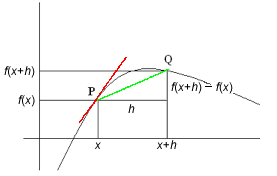
\includegraphics[width=2.5in]{img/derivative} \\
slope of the \textcolor{green}{secant line} through P and Q $=\frac{f(x+h)-f(x)}{h}$\\
slope of the \textcolor{red}{tangent line} through P $=f'(x)$%\end{small}
\end{figure}
\end{frame}


\begin{frame}
\frametitle{Economic example}
%\begin{small}
In economics, the following \textcolor{blue}{crude approximation} is used
$$
f'(x) \approx f(x+1)-f(x).
$$
Then the derivative is often called the \textcolor{blue}{marginal}, since it is a good approximation of the marginal change of $f$ at $x$. The less curved the graph of $f$, the better approximation.

\vskip 12pt

\textcolor{blue}{Example:} Consider a \textcolor{blue}{cost function} $f(x)$ which measures the cost of manufacturing $x$ units of an output. Then the marginal cost is the cost of making one more unit.
\vskip 12pt
 If the change in the amount is $\Delta x$ instead of one unit, then one can use the approximation
$$
f'(x)\Delta x \approx f(x+\Delta x)-f(x).
$$
%In differential notation
%$$
%f'(x) dx \approx df.
%$$
%
%
%\end{small}
\end{frame}

\begin{frame}
\frametitle{Differentiation rules}
%\begin{small}
\textcolor{blue}{Derivatives of elementary functions:}
\begin{enumerate}
\item $f(x)=c$, $\;$ $f'(x)=0$, where $c$ is a constant.
\item $f(x)=x^n$, $\;$ $f'(x)=nx^{n-1}$, where $n$ is a positive  integer.
\item $f(x)=x^{\alpha}$, $\;$ $f'(x)=\alpha x^{\alpha-1}$, where $\alpha \in \R$ and $x>0$.
\item $f(x)=\log(x)$, $\;$ $f'(x)=\frac{1}{x}$, $x>0$.
\item $f(x)=\sin(x)$, $\;$ $f'(x)=\cos(x)$.
\item $f(x)=\cos(x)$, $\;$ $f'(x)=-\sin(x)$.
\item $f(x)=e^x$, $\;$ $f'(x)=e^x$.
\item $f(x)=a^x$, $\;$ $f'(x)=a^x \log a$, $a>0$.
\end{enumerate}

\begin{tiny}Proof of 8: $(a^x)'=(e^{x\log(a)})'=a^x \log(a)$ (by the chain rule)\end{tiny}

\begin{tiny} Example of 3: $(\sqrt{x})'=\frac{1}{2\sqrt{x}}$ \end{tiny}



%\end{small}
\end{frame}



\begin{frame}
\frametitle{Differentiation rules}
%\begin{small}



\textcolor{blue}{Theorem:} If $f$ and $g$ are \textcolor{blue}{differentiable}, then so are $f+g$,
$fg$ and $f/g$ (the last one provided that $g(x) \neq 0$), and

\begin{itemize}
\item $(f+g)'(x)=f'(x)+g'(x)$,
\item $(fg)'(x)=f'(x)g(x)+g'(x)f(x)$,\qquad[Leibniz rule]
\item $\left(\frac{f}{g}\right)'(x)=\frac{f'(x) g(x)-g'(x)f(x)}{g^2(x)}$.
\end{itemize}
%\begin{tiny} The second and third formulas follow from the chain rule \end{tiny}



%\end{small}
\end{frame}






\begin{frame}{Differentiation rules}
\begin{alertblock}{Chain rule: }
	Let $f,g$ be two continuous functions. If $f$
is differentiable at $x \in D_f$, and $g$ is differentiable at $f(x)\in D_g$,
then $h=g \circ f$ is differentiable at $x$ and 
$$
h'(x)=g'(f(x)) f'(x).
$$
\end{alertblock}

\textcolor{blue}{Example 1:} The production cost of a firm  is
$$
C=f(x)=4+\log(x+1)+\sqrt{3x+1}.
$$
By the chain rule
$$
C'=f'(x)=\frac{1}{x+1}+\frac{3}{2\sqrt{3x+1}}.
$$
\begin{tiny}
 If the production increases from 133 to 134, the production cost increases  by $C'(133) \approx 0.08246$ units.
\end{tiny}
\end{frame}


\begin{frame}{Example 2: $h(x)=u(x)^{v(x)}$ with $u(x)>0$}
\small
We use \textbf{logarithmic differentiation}. Define
\[
h(x)=u(x)^{v(x)},\qquad u(x)>0.
\]
Take logs:
\[
\ln h(x) = v(x)\,\ln u(x).
\]
Differentiate both sides (product + chain rules):
\[
\frac{h'(x)}{h(x)} 
= v'(x)\,\ln u(x)\;+\;v(x)\,\frac{u'(x)}{u(x)}.
\]
Multiply by $h(x)$:
\[
\boxed{\;h'(x)=u(x)^{v(x)}
\Big(v'(x)\,\ln u(x) + v(x)\,\frac{u'(x)}{u(x)}\Big).\;}
\]

\medskip
\textbf{Checks (special cases).}
\begin{itemize}
\item If $v(x)\equiv c$ (constant): $h(x)=u(x)^c\Rightarrow 
h'(x)=c\,u(x)^{c-1}u'(x)$.
\item If $u(x)\equiv a>0$ (constant): $h(x)=a^{v(x)}\Rightarrow 
h'(x)=a^{v(x)}\ln(a)\,v'(x)$.
\end{itemize}
\end{frame}


\begin{frame}{Differentiation rules}
%\begin{small}
\textcolor{blue}{Theorem (derivative of the inverse):} Let $f$ be a strictly monotone continuous function  differentiable at $x \in D_f$. Then the inverse $f^{-1}$ is differentiable at $y=f(x)$ if and only if $f'(x) \neq 0$, and in this case
$$
(f^{-1})'(y)=\frac{1}{f'(x)}=\frac{1}{f'(f^{-1}(y))}.
$$
\begin{tiny} Proof : since $f^{-1}(f(x))=x$, by the chain rule $(f^{-1})'(f(x))f'(x)=1$ \end{tiny}
\vskip 11pt
\textcolor{blue}{Example:}  $f(x)=e^x$, $f'(x)=e^x > 0$, therefore, $(\log)'(y)=\frac{1}{y}$ for all $y>0$.
\vskip 11pt
\textcolor{blue}{Higher-order derivatives:} If $f'$ is differentiable,  its derivative is called the \textcolor{blue}{second derivative} of $f$ and  denoted $f''$. Similarly, we can define \textcolor{blue}{higher-order derivatives}, and $f^{(n)}$ is called the $n$th derivative of $f$. If $f^{(n)}$ is continuous, we say that $f$ is $n$ times \textcolor{blue}{continuously differentiable} or \hl{$C^{n}$} for short.


%\end{small}
\end{frame}

\begin{frame}
\frametitle{Limits}
%\begin{small}
 \textcolor{blue}{Theorem (L'H\^opital's rule):} Let $f,g$ be  two $C^1$ functions in $(a,b)$ with $g' \neq 0$
in $(a,b)$. Assume that one of the next hypothesis is satisfied:
\begin{itemize}
\item[(a)] $\lim_{x \rightarrow x_0} f(x)=\lim_{x \rightarrow x_0} g(x)=0$.
\item[(b)] $\lim_{x \rightarrow x_0} f(x)=\lim_{x \rightarrow x_0} g(x)=\infty$ or $-\infty$.
\end{itemize}
Then,
$$
\lim_{x \rightarrow x_0} \frac{f(x)}{g(x)}=\lim_{x \rightarrow x_0} \frac{f'(x)}{g'(x)}.
$$
\begin{tiny} The proof uses the Mean value theorem (on slide~\ref{mv}) \end{tiny}

\begin{tiny}\textcolor{blue}{Remark:} $x$ can be $\infty$ or $-\infty$ and $\lim_{x \rightarrow x_0} \frac{f'(x)}{g'(x)}$
can be $\infty$ or $-\infty$.\end{tiny}
\vskip 12pt
\textcolor{blue}{Example:} 
\begin{equation*}
\begin{split}
\lim_{x \rightarrow 0} (1+x)^{1/x}=\lim_{x \rightarrow 0} e^{\log (1+x)^{1/x}}=
e^{\lim_{x \rightarrow 0} \frac{\log (1+x)}{x}}=e^{\lim_{x \rightarrow 0} \frac{1}{1+x}}=e
\end{split}
\end{equation*}
\begin{tiny}We have used l'H\^opital's rule in the third equality and the last property in page 28 in the second one.\end{tiny}


%\end{small}
\end{frame}


\begin{frame}
\frametitle{Monotonicity}
%\begin{small}
\textcolor{blue}{Theorem:} Consider $f$ differentiable in $(a,b)$. Then 
\begin{enumerate}
\item $f$ is increasing on $[a,b]$
$\Longleftrightarrow$  $f'\geq 0$ on $(a,b)$.
\item $f$ is decreasing on $[a,b]$ 
$\Longleftrightarrow$ $f'\leq 0$ on $(a,b)$. 
\item $f$ is constant on $[a,b]$ $\Longleftrightarrow$ $f'=0$ on $(a,b)$.
\item If $f'>0$ on $(a,b)$, then $f$ is strictly increasing on $[a,b]$.
\item If $f'<0$ on $(a,b)$, then $f$ is strictly decreasing on $[a,b]$.
\end{enumerate}
\begin{tiny}Observe that $f(x)=x^3$ is strictly increasing but $f'(0)=0$, so the converse in 4. and 5. is not necessarily true.\end{tiny}
\vskip 12pt
\textcolor{blue}{Example:} $f(x)=\frac{x^3}{3}+2x^2+3x+1.$ We have
$$
f'(x)=x^2+4x+3=(x+1)(x+3).
$$
Therefore, $f$ is strictly increasing on $(-\infty, -3]$ and $[-1, \infty)$, while $f$ is strictly decreasing on $[-3,-1]$.

\begin{tiny}This implies that $-3$ is a local max and $-1$ is a local min (see next slide). 
However, there are no global optima since $\lim_{ x \rightarrow \pm \infty} f(x)=\pm \infty$.  \end{tiny}


%\end{small}
\end{frame}








\begin{frame}
\frametitle{Optimal points: 1st order conditions}
%\begin{small}
Let $f:D \rightarrow \R$. A point $x_0 \in D$ is called a \textcolor{blue}{local max} (resp. \textcolor{blue}{local min}) of $f$ if there is an interval $(a,b) \subset D$ containing $x_0$ such that $$f(x)\leq f(x_0), \quad \text{ for all } x \in (a,b)$$ (resp. $f(x) \geq f(x_0)$)
\vskip 12pt
We say that $x_0$ is a \textcolor{blue}{global max} (resp. \textcolor{blue}{global min}) if $$f(x)\leq f(x_0)\quad \text{for all } x \in D$$ (resp. $f(x) \geq f(x_0)$) 

\begin{tiny} Boundary points are typically not considered as local max or min, we call a max or a min an optimum  \end{tiny}

 




%\end{small}
\end{frame}

\begin{frame}{Optimal points}
\begin{figure}
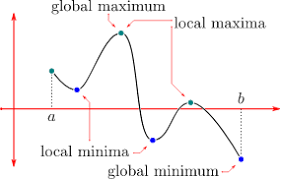
\includegraphics[width=2.5in]{img/max_min} 
\end{figure}
\end{frame}

\begin{frame}{Optimal points: 1st order conditions}
 \textcolor{blue}{Theorem:} If $f$ has a local optimum at $x \in (a,b)$ and $f$ is differentiable at $x$, then $f'(x)=0$.
\vskip 12pt
\textcolor{blue}{Remark:} The condition is \textcolor{blue}{only necessary}, for example if $f(x)=x^3$, $f'(0)=0$ but $0$ is not a local max or min.
\vskip 12pt
Points $x$ such that $f'(x)=0$ are called \textcolor{blue}{stationary points}.
\vskip 12pt
\textcolor{blue}{Theorem:} Let $f$ differentiable and $x \in (a,b)$ a stationary point. If there exists an interval $(a^{\ast}, b^{\ast})$ around $x$ such that the function is strictly increasing (resp. decreasing) to the left of $x$ and strictly decreasing (resp. increasing) to the right of $x$, then $x$ is a local max (resp. min).
\end{frame}


\begin{frame}{Economic example}
%\begin{small}
Suppose you own a property whose market value will be $V(t)$ pesos $t$ years from now. If the interest rate is $R$, this means that the present value is $P(t)=V(t) e^{-Rt}$.
What is the optimal time $t_0$ to sell this property ? We maximize its present value with respect  to $t$.
\vskip 12pt
The \textcolor{blue}{first order condition} is
$$
P'(t)=(V(t) e^{-Rt})'=V'(t) e^{-Rt}-RV(t) e^{-Rt}=0 \Rightarrow \frac{V'(t)}{V(t)}=R
$$ 
The optimal time to sell is when the rate of change of $V$ equals the interest rate you can earn in the bank.
\vskip 12pt

 \textcolor{blue}{Example}: If $V(t)=10000e^{\sqrt{t}}$and $R=6\%$ then the present value is 
$$
P(t)=10000e^{\sqrt{t}-0.06 t}.
$$
The optimal time to sell is $t \approx 69.44$, which is the global max of $P$ on $[0, \infty)$.


%\end{small}
\end{frame}

\begin{frame}
\frametitle{Plot of the present value $P(t)$}


\begin{figure}
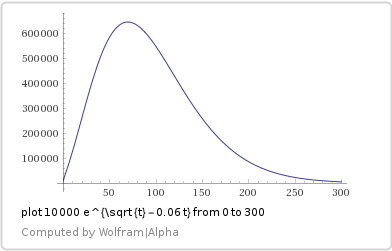
\includegraphics[width=3.5in]{img/plot} 
\end{figure}
%\begin{small}To check  that  a  local optimum is global we need to look at the value  of  the  function at the  extreme points of the domain. 

Here $P(0)=10000$ and $\lim_{t \rightarrow \infty} P(t)=0$.%\end{small}
\end{frame}

\begin{frame}
\frametitle{Optimal points: 2nd order conditions}
%\begin{small}
\textcolor{blue}{Theorem:} Let $f:(a,b) \rightarrow \R$ a $C^n$ function, and $x \in (a,b)$ a stationary point. If
$$
f'(x)=f''(x)=\dots=f^{(n-1)}(x)=0, \quad \text{and} \quad f^{(n)}(x) \neq 0,
$$
where $n$ is \textcolor{blue}{even}, \begin{tiny} (typically $n=2$)\end{tiny} then:
\begin{enumerate}
\item If $f^{(n)}(x)<0$, the $x$ is a local max.
\item If $f^{(n)}(x)>0$, the $x$ is a local min.
\end{enumerate}

\textcolor{blue}{Example:} Find the optimal points of $f(x)=\frac{\log^2 3x}{x}$, $x>0$.
$$
f'(x)=\frac{(2-\log 3x)\log 3x}{x^2}
$$
$f'$ has two zeroes at $x_1=1/3$ and $x_2=e^2/3$.
$$
f''(x)=\frac{2(1-3\log3x+\log^23x)}{x^3}
$$
Since $f''(x_1)>0$ and $f''(x_2)<0$, $x_1$ is a local min and $x_2$ is a local max.
%\end{small}
\end{frame}


\begin{frame}
\frametitle{Plot of $f(x)=\frac{\log^2 3x}{x}$, $x>0$}

\begin{figure}
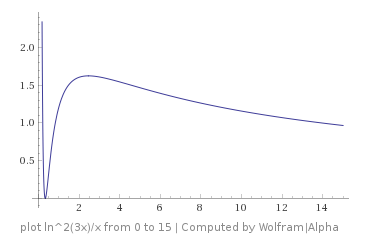
\includegraphics[width=3.5in]{img/ima} 
\end{figure}
%\begin{small}Since $\lim_{x \rightarrow \infty} f(x)=0$, $\lim_{x \rightarrow 0} f(x)=\infty$
and $f(x_1)=0$, $f(x_2)>0$, $x_1$ is a global min but there a no global max.%\end{small}
\end{frame}



\begin{frame}
\frametitle{Convexity and concavity}
%\begin{small}
 \textcolor{blue}{Theorem:} Let $f$ be a twice differentiable on $(a,b)$. Then:
\begin{enumerate}
\item $f$ is convex (concave) on $[a,b]$ if and only if $f''(x)\geq 0$  ($f''(x)\leq 0$) for all $x \in (a,b)$.
\item If $f''(x)> 0$ ($f''(x)< 0$) for all $x \in (a,b)$, then $f$ is strictly convex (concave).
\end{enumerate}



 \textcolor{blue}{Example:} $f(x)=\frac{2x}{x^2+1}$.
$$
f'(x)=\frac{2(1-x^2)}{(x^2+1)^2}\qquad f''(x)=\frac{4(x^3-3x)}{(x^2+1)^3}.
$$
Then, $f$ is strictly convex on $[-\sqrt{3},0] \cup [\sqrt{3}, \infty)$ and strictly concave on $(-\infty, -\sqrt{3}] \cup [0, \sqrt{3}]$.
 \vskip 11pt
 \textcolor{blue}{Theorem:} If $f$ and $g$ are convex (or concave), then $f \circ g$ is convex (or concave).
 
\textcolor{blue}{Example:} $f(x)=e^{x^2}$ is strictly convex on $[0, \infty)$.

%\end{small}
\end{frame}

\begin{frame}
\frametitle{Plot of $f(x)=\frac{2x}{x^2+1}$}

\begin{figure}
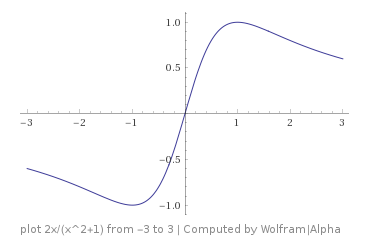
\includegraphics[width=3.5in]{img/ima1} 
\end{figure}

%\begin{small}The points 0, $\sqrt{3}$ and $-\sqrt{3}$ are inflexion points. The points $1$ and $-1$ are global max and min since $\lim_{x \rightarrow \infty} f(x)=0$ and $\lim_{x \rightarrow -\infty} f(x)=0$.%\end{small}
\end{frame}

\begin{frame}
\frametitle{Convexity and concavity}
%\begin{small}
Let $f$ be a twice differentiable on $(a,b)$. A point $x \in (a,b)$ is called an \textcolor{blue}{inflexion point} if $f$ changes at $x$ from being concave to convex, or vice versa.
\vskip 12pt
\textcolor{blue}{Theorem:} Let $f:D_f \rightarrow \R$ $C^n$ on $(a,b)$. $f$ has an inflexion point at $x \in (a,b)$ if and only if
$$
f''(x)=\dots=f^{(n-1)}(x)=0, \quad \text{and} \quad f^{(n)}(x) \neq 0,
$$
where $n$ is \textcolor{blue}{odd}.

\begin{tiny} (typically $n=3$, that is, $f''(x)=0$ and $f'''(x) \neq 0$)\end{tiny}
\vskip 12pt
 \textcolor{blue}{Example:} $f(x)=x^3$, $f'(x)=3x^2$, $f''(x)=6x$, $f'''(x)=6>0$, 
so 0 is an inflexion point.


%\end{small}
\end{frame}


\begin{frame}[label=mv]{Mean-value theorem}
\begin{alertblock}{Mean value theorem:}
	If $f$ is continuous on $[a,b]$ and differentiable on $(a,b)$,
then there exists $c \in (a,b)$ such that
$$
f'(c)=\frac{f(b)-f(a)}{b-a}\qquad\mbox{(or}\;\; f(b)=f(a)+f'(c)(b-a)\mbox{)}.
$$
\end{alertblock}
\begin{tiny}Proof: Set $h(x)=(f(b)-f(a))x-(b-a)f(x)$, and show that since $h(a)=h(b)$ it has a local max or min. \end{tiny}
\vskip 12pt
\textcolor{blue}{Geometric interpretation:} $\frac{f(b)-f(a)}{b-a}$ is the \textcolor{blue}{slope of the secant line} connecting 
the points $(a, f(a))$ and $(b,f(b))$. Thus, the mean value theorem says that there exists $c \in (a,b)$, such that the tangent line to $f$ at $c$ is parallel to the secant line.
\end{frame}

\begin{frame}
\frametitle{Geometry of the mean-value theorem}
Recall: \ldots there exists $c \in (a,b)$ such that
$$
f'(c)=\frac{f(b)-f(a)}{b-a}\qquad\mbox{(or}\;\; f(b)=f(a)+f'(c)(b-a)\mbox{)}.
$$
\begin{figure}
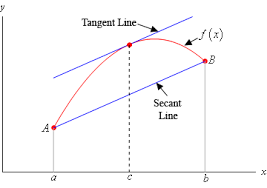
\includegraphics[width=2.5in]{img/secant} 

\end{figure}


\end{frame}

\begin{frame}{Taylor formula}
\textcolor{blue}{Theorem (Taylor's formula of order $n$):} Let $f$ be $n+1$ times differentiable on $(a,b)$,
 and let $x_0 \in (a,b)$ given. Then, for any $x \in (a,b)$,
 if $n=1$,
$$ f(x)=f(x_0)+f'(x_0)(x-x_0)+\text{error}.$$
If  $n=2$
$$f(x)=f(x_0)+f'(x_0)(x-x_0)+\frac{f''(x_0)}{2!}(x-x_0)^2+\text{error}.$$
If  $n>2$,
 \begin{equation*} \begin{split}
 f(x)=\textcolor{DarkRed}{f(x_0)+f'(x_0)(x-x_0)+\frac{f''(x_0)}{2!}(x-x_0)^2+
\frac{f^{(n)}(x_0)}{n!}(x-x_0)^n}+\text{error}.
 \end{split}
 \end{equation*}
 
 
  The error is small if $x$ is close to $x_0$, therefore, this theorem says that differentiable functions may be \textcolor{blue}{locally approximated
 by a polynomial} called the \textcolor{DarkRed}{Taylor polynomial}.
%\end{small}
\end{frame}

\begin{frame}{Taylor's error}
\begin{alertblock}{The remainder term has the form}
\[
R^y_n(x) = \frac{f^{(n+1)}(y)}{(n+1)!}\,(x-x_0)^{n+1}\qquad\mbox{for some }y \mbox{ between $x_0$ and $x$}.
\]
\end{alertblock}
\medskip
If $f^{(n+1)}$ is bounded on $(a,b)$ by a constant $M$, then
\[
|R^y_n(x)| \le \frac{M}{(n+1)!}\,|x-x_0|^{n+1}.
\]
\textcolor{blue}{Example:} For $f(x)=\log(x)$ around $x_0=1$: $
f'(x)=\frac1x$, $f''(x)=-\frac1{x^2}$, $f^{(3)}(x)=\frac{2}{x^3}$.
The degree-$2$ Taylor polynomial is $\log(x) \approx (x-1) - \frac12 (x-1)^2$.
The error term is
\[
R^y_2(x) = \frac{f^{(3)}(y)}{3!}(x-1)^3 = \frac{1}{3y^3}(x-1)^3,
\]
which, for $x>1$, is bounded by $\frac13(x-1)^3$.
\end{frame}

\begin{frame}{What is a European call option?}
\small
A \textbf{European call option} is a contract that gives its owner the right (but not the obligation) 
to \emph{buy} a stock for a fixed \emph{strike price} $K$ at a specific \emph{maturity date} $T$.

\medskip
Payoff at maturity:
\[
\text{Payoff} = \max(S_T - K,\, 0)
\]
- If $S_T > K$: you can buy at $K$ and immediately sell at $S_T$, earning $S_T - K$.
- If $S_T \le K$: you would not exercise the option (payoff is 0).

\medskip
\textbf{Value before maturity:} At time $t<T$, the option has market value $C_t(S_t)$,  
depending on:
\begin{itemize}
\item the current stock price $S_t$,
\item time to maturity $T-t$,
\item volatility, interest rates, and other market factors.
\end{itemize}
%
%\begin{center}
%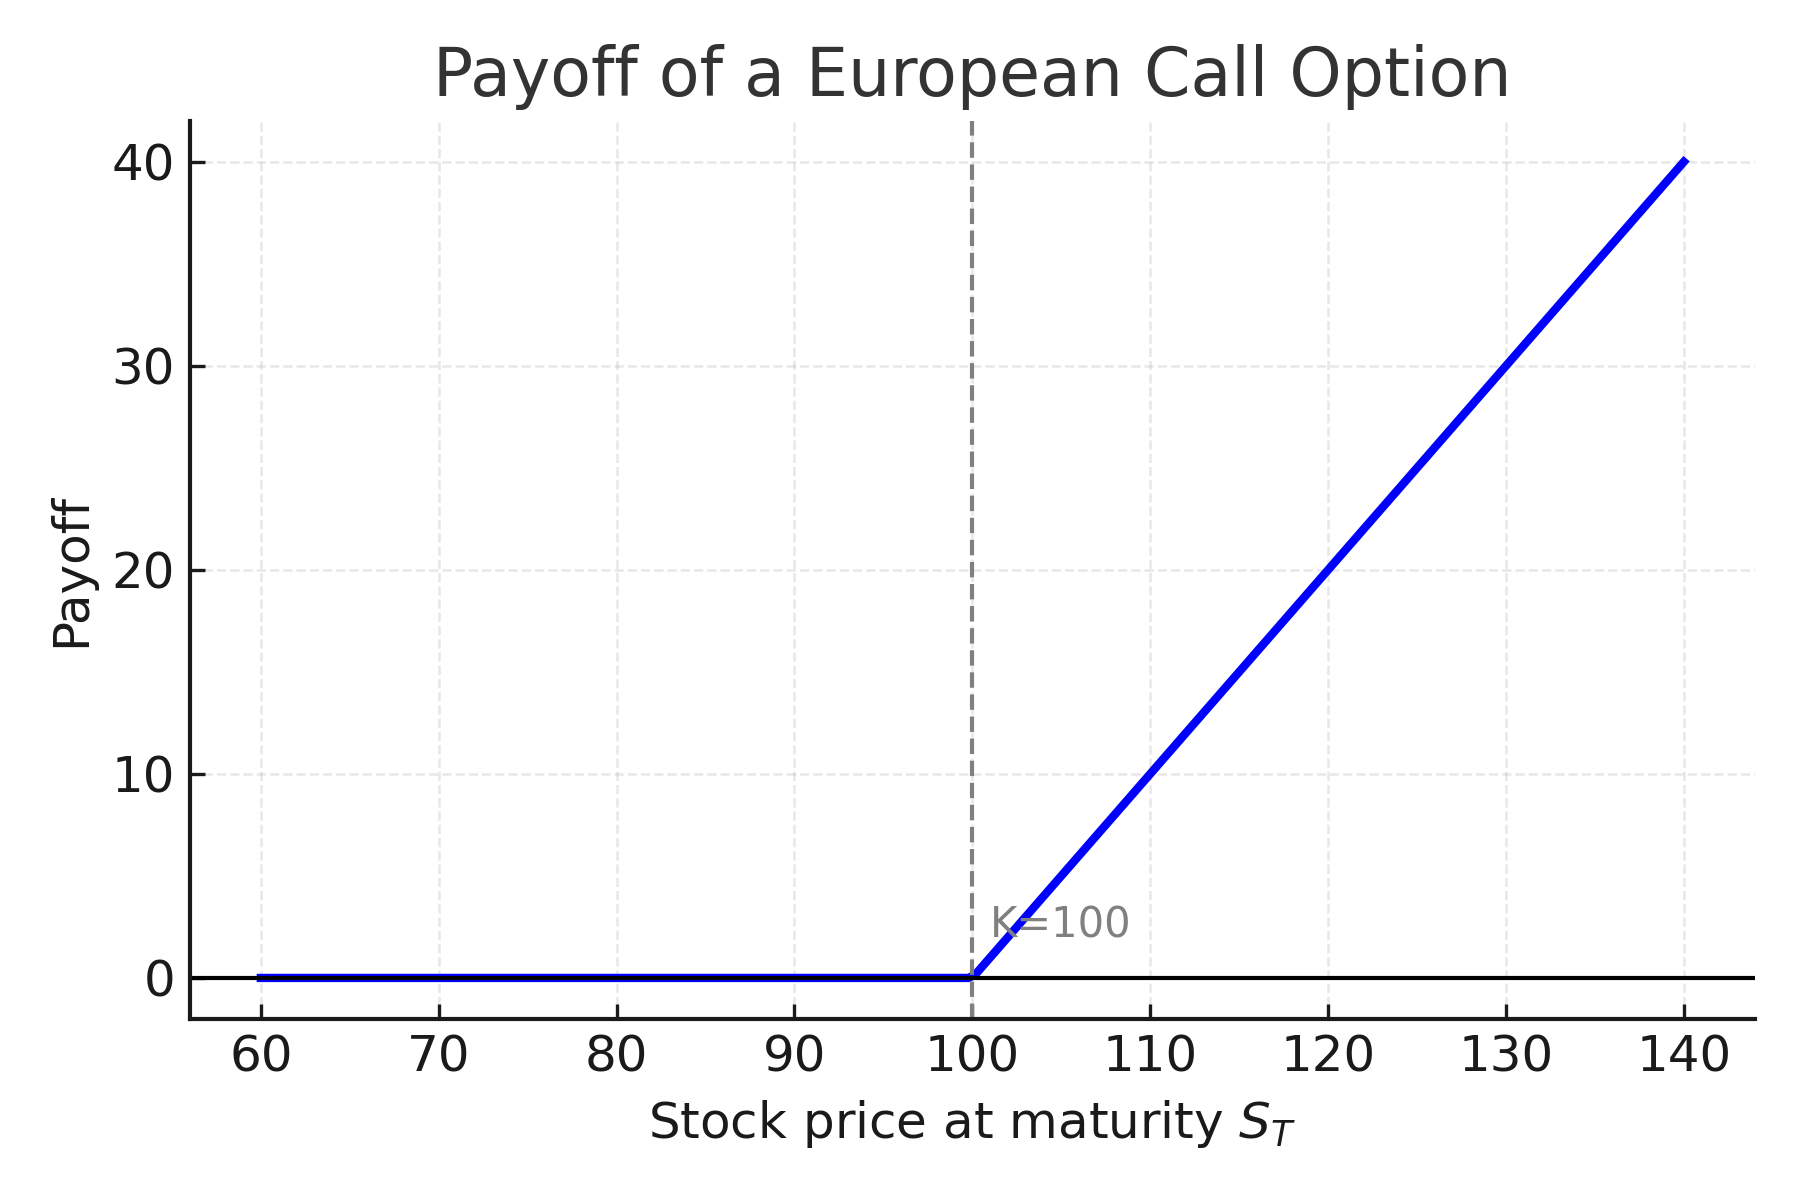
\includegraphics[scale=.3]{img/callpayoff.png}
%\end{center}
\end{frame}


\begin{frame}{Reducing risk with a hedge}
\small
Suppose at $t=0$ we:
\begin{itemize}
\item \textbf{Own one call option} with value $C_0(S_0)$.
\item \textbf{Sell $\Delta_0$ shares} of the stock, where 
$\Delta_0 = C_0'(S_0)$ measures how much the option value changes per unit change in the stock price.
\end{itemize}

The total portfolio value is:
\[
\Pi_0 = C_0(S_0) - \Delta_0 S_0.
\]

\medskip
If the stock price changes from $S_0$ to $S_0 + x$ (small $x$), the new portfolio value is:
\[
\Pi_1 = C_0(S_0 + x) - \Delta_0 (S_0 + x).
\]

\medskip
\textbf{Profit or loss} from this price move:
\[
V_0 = \Pi_1 - \Pi_0 = C_0(S_0+x) - C_0(S_0) - \Delta_0\,x.
\]
%\begin{center}
%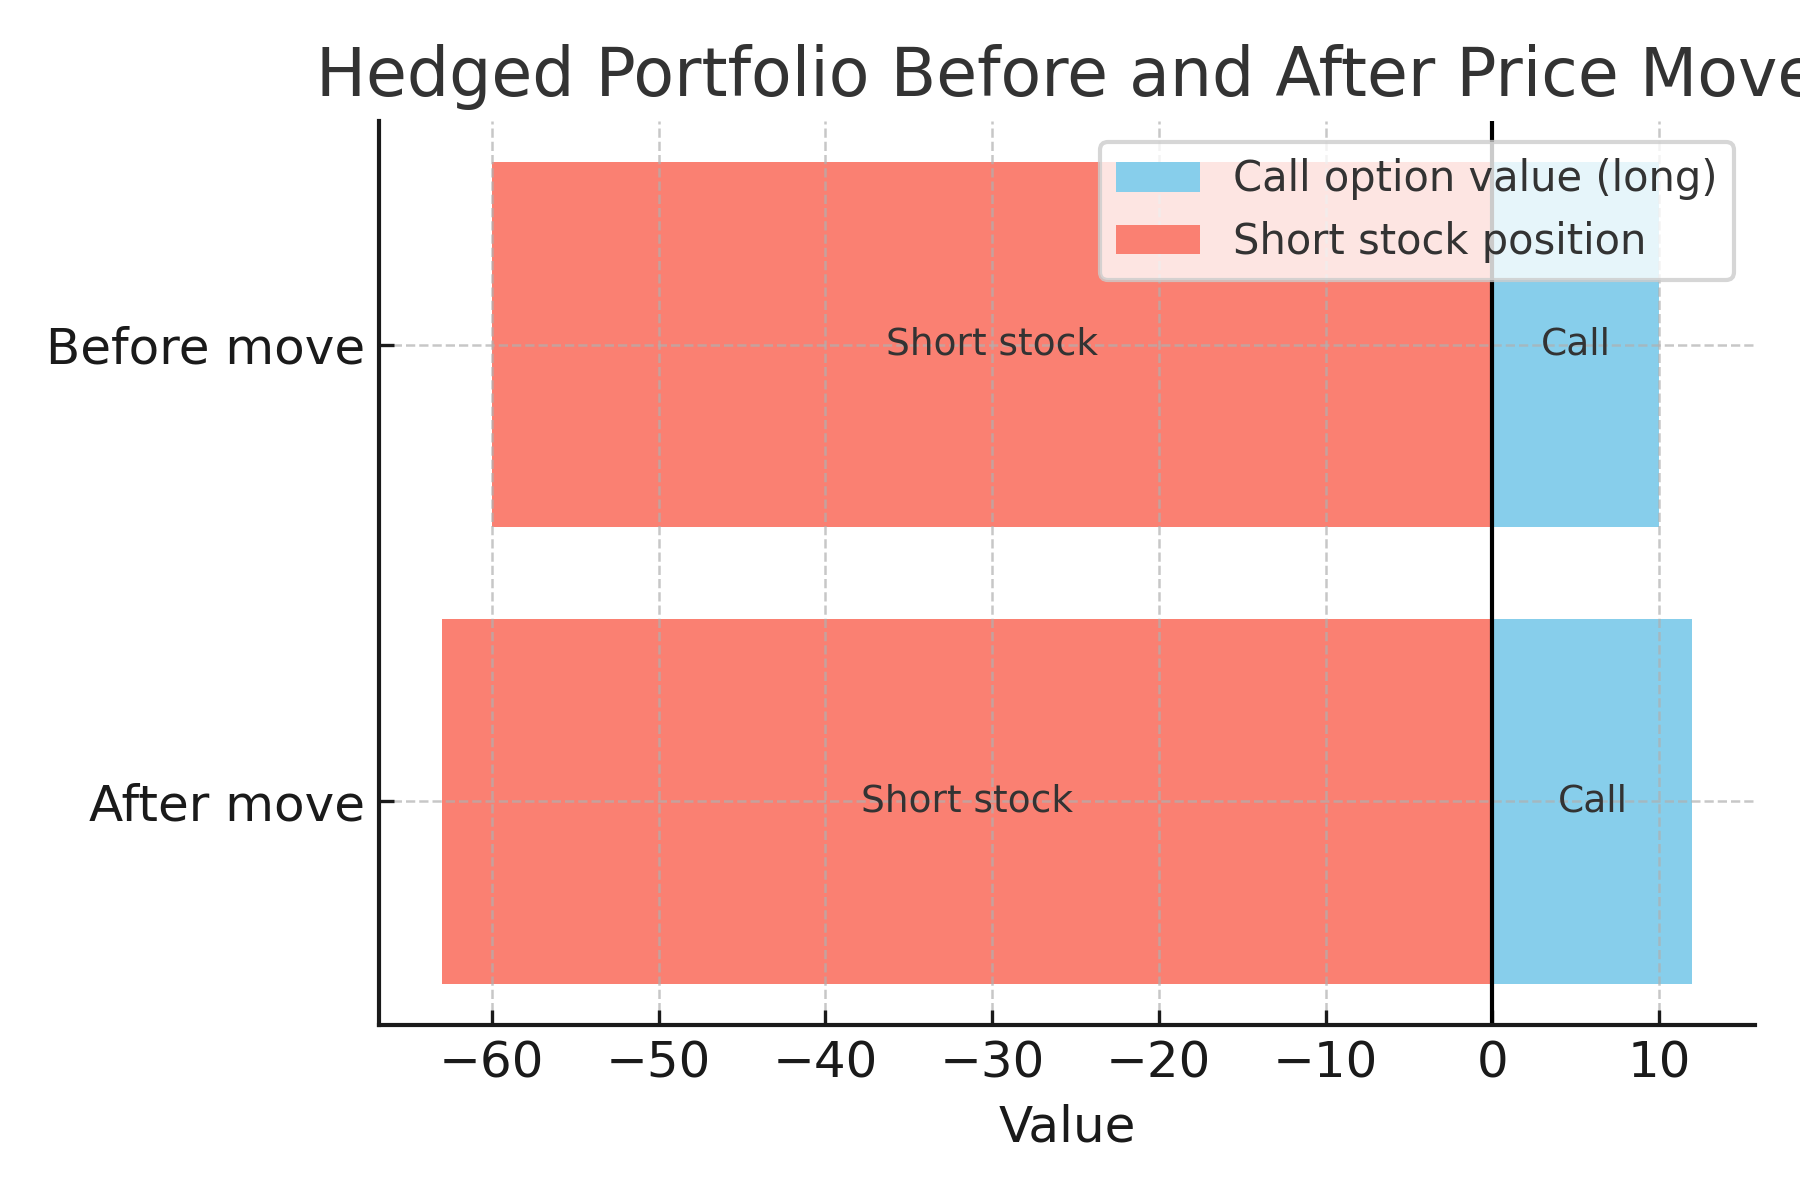
\includegraphics[width=0.6\linewidth]{img/hedgedportfolio.png}
%\end{center}
\end{frame}

\begin{frame}{Taylor approximation and remaining risk}
\small
Using Taylor's formula for $C_0(S_0+x)$:
\[
C_0(S_0+x) = C_0(S_0) + \Delta_0\,x + \frac12 \Gamma_0\,x^2 + O(x^3),
\]
where $\Gamma_0 = C_0''(S_0)$ measures how fast the Delta changes.

\medskip
Substitute into $V_0$:
\[
V_0 = \frac12 \Gamma_0\,x^2 + O(x^3).
\]

\textbf{Interpretation:}
\begin{itemize}
\item Choosing $\Delta_0$ as above removes the \emph{first-order} effect of small price changes.
\item The remaining risk is due to the curvature of $C_0(S)$, called \textbf{Gamma risk}.
\end{itemize}
%
%\medskip
%\textbf{Example:} 1-month call option, $K=100$, $S_0=100$, volatility 20\%.
%\begin{figure}
%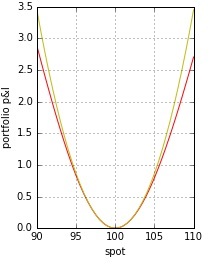
\includegraphics[width=1in]{img/deltahb}
%\end{figure}
\end{frame}
\end{document}
